\section{General continuous piecewise linear functions as a DNN}
\subsection{Lattice representation of CPWL}

We say a function $f:\mathbb{R}^n \to \mathbb{R}$ is continuous piecewise linear (CPWL) if there exists a finite set of polyhedra whose union is $\mathbb{R}^n$, and $f$ is affine linear over each polyhedron (note that the definition automatically implies continuity of the function because the affine regions are closed and cover $\mathbb{R}^n$, and affine functions are continuous). The number of pieces of $f$ is the number of maximal connected subsets of $\mathbb{R}^n$ over which $f$ is affine linear (which is finite).

\begin{figure}[!ht]
\centering
	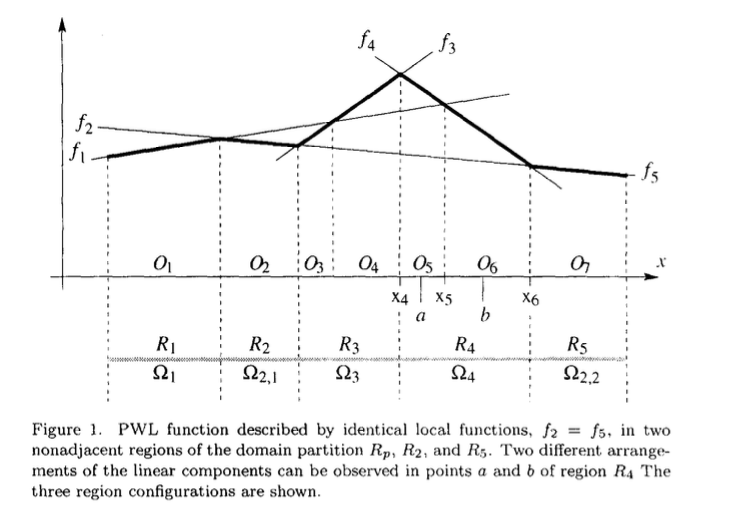
\includegraphics[width=0.6\textwidth]{6DL/figures/latticePWL.png}   
	\caption{Unique order regions.} 
	\label{fig:latticePWL}
\end{figure}
Figure \ref{fig:latticePWL} shows a CPWL function with unidimensional domain that has a domain partition generated by $4$ boundaries. The result is a set of $5$ regions and the corresponding set of $5$ local functions, two of which are identical, $f_2$ and $f_5$. In the case of a model described in terms of the local functions. 

The arrangements in ascending order of the linear functions in the points $a$ and $b$ of region $R_4$ are respectively, ($f_2 = f_5 < f_1 < f_4 < f_3$) and ($f_2= f_5 < f_4 < f_1 < f_3$). We note that the intersection of the linear functions fland f4occurs at point x5, an inner point of $R_4$. Given the importance of the order arrangement when dealing with models based on the local functions, the division of region $R_4$ into two subregions is practically meaningful.

Any intersection of linear functions produces a change of order arrangement. So, if we consider every intersection of local functions, the resulting domain partition will be formed by connected, and convex regions with a unique order arrangement. It should be noted that some of those intersections might not correspond to any boundary of the PWL function.  

We introduce a domain partition that will have unique order on each subdomain \cite{tarela1999region}.
\begin{definition}
	Let $f:\mathbb{R}^n\to\mathbb{R}$ be a continuous piecewise linear function with m distinct local functions $l_i$, $1\le i\le m$. Consider the intersections between local functions, those intersections with some noticed segments in $f$ will be called visible boundaries, and those boundaries corresponds to the set of functions $\{\phi_{\lambda_v}\}$. The rest of intersections occurring inside the domain will be called hidden boundaries and noted as $\{\phi'_{\lambda_h}\}$. A \textbf{unique-order region} is each region of the domain partition produced by the boundary configuration $\{\phi_{\lambda_v}\}\bigcup\{\phi'_{\lambda_h}\}$.
\end{definition}

\bigskip
The unique-order regions have the following characterizations:
\begin{itemize}
	\item The domain of $f$ is divided into $M$ unique-order regions.
	\item The local function associated to two unique-order regions may be identical.
	\item The unique-order regions are convex.
	\item A unique-order region has the same rearrangement in ascending order of the values of the $m$ local functions in all its points.
\end{itemize}

\begin{remark}
	If $m$ is the number of distinct linear components of $f$, then the maximum number of rearrangements in ascending order is $m!$. However, the number of unique-order regions is in general lower than $m!$, because of the geometric constraints of the problem \cite{wilkinson1963method}. Thus, the different arrangements in $\mathbb{R}^n$ is $Q$, then:
	\begin{equation*}
	\begin{aligned}
	&\mathrm{if}\ 1\le m\le n+1\quad\Rightarrow Q=m!\\
	&\mathrm{if}\ m\ge n+2\quad\Rightarrow (n+1)!<Q<m!
	\end{aligned}
	\end{equation*}
	The number of unique-regions is $M$, then we have $M\le Q$, since only some of these arrangements constitute unique-order regions.
\end{remark}




\begin{lemma}\label{lem:1dlattice}
	If $p(t)$ is a continuous piecewise linear function. And the unique-order region partition is
	$$0 = t_0 < t_1 < ... < t_{r+1} = 1$$
	and the linear function in $[t_i,t_{i+1}]$ is $l_i(t) = k_i t+b_i$. And parameter satisfied 
	$$ b_0 > b_r,\qquad k_0 + b_0 > k_r + b_r $$
	which means
	$$l_0(t)> l_r(t)\quad \mbox{in}\quad [t_0,t_1]$$
	$$l_0(t)> l_r(t)\quad \mbox{in}\quad [t_r,t_{r+1}]$$
	Then, exist $l_p(t) = k_p t+ b_p$, such that
	$$b_p \ge b_0,\qquad k_p+b_p\le k_r+b_r$$  
	That's to say
	$$l_0(t)\le l_p(t)\quad \mbox{in}\quad [t_0,t_1]$$
	$$l_p(t)\le l_r(t)\quad \mbox{in}\quad [t_r,t_{r+1}]$$
\end{lemma}
\begin{figure}[th]
	\centering
	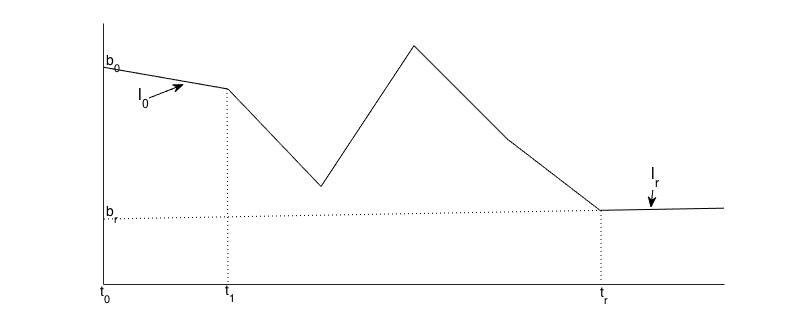
\includegraphics[width=0.7\linewidth]{6DL/pic/fig1}
	\caption{}
\end{figure}

\begin{proof}
	
	Let $k_p=\min\{k_i\}$, $\Delta t_i=t_{i+1}-t_i$. 
	Since here we only have linear functions, so we can represent each point $(t_i,y_i)$ by using $k_i$'s and $\Delta t_i$'s.
	Then the point $(t_p,b_0+\sum_{i=0}^{p-1}k_i\Delta t_i)$ is on $y=k_p t+b_p$, so we can represent $b_p$ as following:
	$$b_p=b_0+\sum_{i=0}^{p-1}k_i\Delta t_i-k_p t_p=b_0+\sum_{i=0}^{p-1}(k_i-k_p)\Delta t_i$$
	Since here $k_p$ is the minimum, we have:
	$$b_p=b_0+\sum_{i=0}^{p-1}(k_i-k_p)\Delta t_i\ge b_0$$		
	And
	\begin{equation*}
	\begin{aligned}
	k_p+b_p&=k_p+b_0+\sum_{i=0}^{p-1}(k_i-k_p)\Delta t_i\\
	k_r+b_r&=k_r+b_0+\sum_{i=0}^{r-1}(k_i-k_p)\Delta t_i\\
	(k_r+b_r)-(k_p+b_p)&=k_r-k_p+\sum_{i=p}^{r-1}(k_i-k_p)\Delta t_i\ge 0
	\end{aligned}
	\end{equation*}
	which means we find the desired pair of $k$ and $p$.
	Notice here $k_p\ne k_0$ and $k_p\ne k_r$ by the assumptions in the lemma. This completes the proof.
	
\end{proof}	


\bigskip		
\begin{theorem}\label{PWLtoRelu}
	For every continuous piecewise linear function $f:\mathbb{R}^n\to\mathbb{R}$ with finite pieces defined by the distinct local linear functions $l_i$, $1\le i\le m$ and $\{\Omega_k\}_{k=1}^M$ be the unique-order subdomains. Then there exist finite non-empty subsets of $\{1,2,\dots,m\}$, say $s_k$, $1\le k\le M$, such that 
	\begin{equation}
	f(x)=\max_{1\le k\le M}\{\min_{i\in s_k} l_i\},
	\end{equation}
	here $s_k=\{i: l_i\ge l_k\ \mathrm{on}\ \Omega_{k}\}$.
\end{theorem}


\begin{proof}
	Let $l_i(x)=f(x)|_{\Omega_k}$. In each $\Omega_{k}$, consider the functions lie completely above $l_k$, and define the convex polynomial
	$$\Phi_{k}=\min_{i\in s_k} l_i.$$
	Define
	$$\Phi(x)=\max_{k} \Phi_{k}(x)$$
	and next we show that $\Phi_{k}(x)\le f(x)$ for all x and every $k$.
	 
	
	For any fixed $k$, if $x_0\in\Omega_{k}$,
	$$
	\Phi_{k}(x_0)=l_k(x_0)= f(x_0).
	$$
	If $x_0\notin\Omega_{k}$, then we suppose $x_0\in \Omega_{k'}$, so 
	$$
	f(x_0)|_{\Omega_{k'}}=l_{k'}(x_0).
	$$ 
	Notice that here we have unique-order region, thus in each $\Omega_i$, the order of $l_k$ and $l_{k'}$ is fixed. There're several situations:
	\begin{enumerate}
		\item  If $l_{k'}(x)\ge l_{k}(x)$ for $x\in \Omega_{k}$, then $l_{k'}$ is a lattice variable in the convex polynomial $\Phi_k$, and so
		$$\Phi_{k}(x_0)\le l_{k'}(x_0)=f(x_0).$$
		\item  If $l_{k'}(x)< l_{k}(x)$ for $x\in \Omega_{k}$, then we consider the domain $\Omega_{k'}$:
		\begin{enumerate}
			\item 
			If $l_{k'}(x)\ge l_k(x)$ for $x\in \Omega_{k'}$. Then on $\Omega_{k'}$,
			\begin{equation*}
			\Phi_{k}(x_0)= l_k(x_0)\le l_{k'}(x_0)=f(x_0)
			\end{equation*}
			\item  
			If $l_{k'}(x)< l_k(x)$ for $x\in \Omega_{k'}$. We take $x\in \Omega_{k}^\circ, x' \in \Omega_{k'}^\circ$. Then we have a path $L(\theta)$, the coordinate of the path is defined as 
			$$
			(x + \theta(x'-x),f(x + \theta(x'-x)))
			$$ 
			with $\theta\in[0,1]$(see Figure~\ref{fig:sec:lattice}). It is just a piecewise linear function with the parameter $\theta$. Notice that the domain partition is unique-order. So if we want to compare the order of the linear function,  we just compare one point value in that region. 
		\begin{figure}[th]
			\centering
			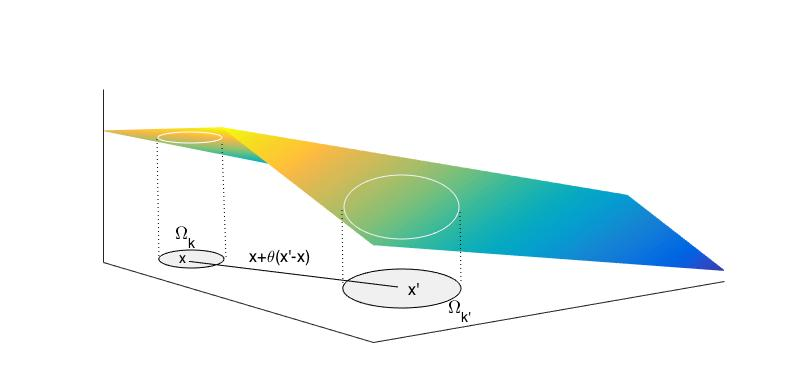
\includegraphics[width=0.7\linewidth]{6DL/pic/fig2}
			\caption{figure}
			\label{fig:sec:lattice}
		\end{figure}
		Then by Lemma \ref{lem:1dlattice}, there must exist $l_t$ with $t\ne k,k'$ and
			\begin{equation*}
			\begin{aligned}
			&l_t\le l_{k'}\quad \mathrm{on}\ \Omega_{k'}\\
			&l_t\ge l_{k}\quad \mathrm{on}\ \Omega_{k}
			\end{aligned}
			\end{equation*}
			Then we should have:
			$$\Phi_{k}(x_0)\le l_t(x_0)\le l_{k'}(x_0)=f(x_0).$$
		\end{enumerate}
	\end{enumerate}
Thus for every $\Phi_{k}$, we have $\Phi_{k}(x)\le f(x)$ for all $x$. It is obvious that  $f(x)\le \Phi_{k}(x)$ for all $x$ since
$$
f(x)=l_k(x)\le \max_k l_k=\max \Phi_k=\Phi(x),\quad \forall x\in \Omega_k.
$$
So 
			$$f(x)=\max_{k}\min_{i\in s_k}\{l_i\}$$
			This is exactly the desired form. Here $|s_k|\le m$, and the number of $\Phi_{k}$ depends on the partition we do. 
\end{proof}




\subsection{General CPWL as a DNN}

Assume that $f:\mathbb{R}^d\to\mathbb{R}$ is a continuous function
that are piecewise linear on $m$ subdomains
$$
\Omega_i, \quad i=1:m.
$$
Namely, on each $\Omega_i$, $f$ is a linear function:
$$
f(x)=f_i(x)=a_i\cdot x+b_i, \quad x\in \Omega_i,
$$
with some $a_i \in \mathbb{R}^d$ and $b_i \in \mathbb{R}$.

Combining Theorem \ref{PWLtoRelu} with Lemma \ref{linearcombine2Relu}, we have the following result.
\begin{theorem}
Every $\mathbb{R}^{d} \rightarrow \mathbb{R}$ ReLU DNN represents a piecewise linear function, and every piecewise linear function $\mathbb{R}^{d} \rightarrow \mathbb{R}$ can be represented by a ReLU DNN with at most $\left\lceil\log _{2}(d+1) \right\rceil+1$ depth.
\end{theorem}
\begin{proof}
It is clear that any function represented by a ReLU DNN is a PWL function. To see the converse, we first note that any PWL function can be represented as a linear combination of piecewise linear convex functions. More formally, by Theorem \ref{PWLtoRelu}, for every piecewise linear function $f: \mathbb{R}^{d} \rightarrow \mathbb{R},$ there exists a finite set of affine linear functions $\ell_{1}, \ldots, \ell_{m}$ and subsets $s_{1}, \ldots, s_{M} \subseteq\{1, \ldots, m\}$ (not necessarily disjoint) where each $s_{i}$ is of cardinality at most $d+1,$ such that
$$
f=\sum_{k=1}^{p} v_{k}\left(\max _{i \in s_{k}} \ell_{i}\right)
$$
where $v_{j} \in\{-1,+1\}$ for all $j=1, \ldots, p .$ Since a function of the form $\max _{i \in s_{j}} \ell_{i}$ is a piecewise linear convex function with at most $n+1$ pieces (because $\left|s_{j}\right| \leq d+1$ ),   any continuous piecewise linear function (not necessarily convex) can be obtained as a linear combination of piecewise linear convex functions each of which has at most $d+1$ affine pieces. Note that $\max \{x, y\}=\frac{x+y}{2}+\frac{|x-y|}{2}$ is implementable by a two layer ReLU network and use this construction in an inductive manner to show that maximum of $d+1$ numbers can be computed using a ReLU DNN with depth at most $\left\lceil\log _{2}(d+1)\right\rceil$.
\end{proof}


For the relationship between ReLU DNNs and general CPWL functions, we have the next theorem with some estimation~\cite{arora2016understanding}. 
\begin{theorem}\label{main0}
	A continuous function $f:\mathbb{R}^d\to\mathbb{R}$ that are piecewise linear on $m$ subdomains $\{\Omega_j\}_{j=1}^m$ can be represented by a ReLU DNN. 
	Furthermore, 
	\begin{enumerate}
		\item the number of  hidden layers  is bounded by 
		\begin{equation}
		\label{layer}
		N_{\rm layer}\le \lceil \log_2(d+1)\rceil.      
		\end{equation}
		\item the number of neurons 
		\begin{equation}
		\label{neurons}
		N_{\rm neuron}=
		\left\{
		\begin{array}{ll}
		\mathcal  O\left(d2^{mM+(d+1)(m-d-1)}\right) & \mbox{ if } m\ge d+1,\\     
		\mathcal O\left(d2^{mM}\right) & \mbox{ if } m< d+1.
		\end{array}
		\right.
		\end{equation}
		here $M$, satisfying $m\le M\le m!$, is the number of subdomains in which $f_i-f_j$ does not change sign. 
	\end{enumerate}
\end{theorem}
Combining Theorem~\ref{main0} with Theorem~\ref{lowerbound}, we have the following corollary regarding the minimal number of layers needed to recover all piecewise linear functions.

\begin{corollary}
	\begin{equation}
	2 \le J_d \le \lceil\log_2(d+1)\rceil.
	\end{equation}
	This also indicates that $\lceil\log_2(d+1)\rceil$ is ``optimal" for $d=2,3$.
\end{corollary}



\endinput 

\section{$\lceil \log(d+1)\rceil$-depth dnn}
Given any $L>n+1$ linear functions, the maximum of these $L$ functions can be represented as the maximum of only $n+1$ linear functions. The next lemma shows that we can reduce the number of functions by one if it is larger than $n+1$. 
Let $l(x,a)=[1\ x^T]a$.
\begin{lemma}\label{reduce}
	For any interger $L$ with $1\le n< L$, $c_0\in\mathbb{R}$ and arbitrary linear function $l_1(x),\dots,l_L(x)$ of $x\in\mathbb{R}^d$, there exist finite groups of $L-1$ linear functions, say $l(x,b_1(k))$, $\dots$,
	$l(x,b_{L-1}(k))$, $1\le k\le K$, and corresponding $c_k\in\mathbb{R}$, $\sigma_k\in\{1,-1\}$ such that
	
	\begin{equation}\label{goal}
	\max\{c_0,l_1,\dots,l_L\} = \sum_{k=1}^{K}\sigma_k\max\{c_k,l(x,b_1(k)),\dots,l(x,b_{L-1}(k))\},
	\end{equation}
	where $K=2^{n+1}-1$.
\end{lemma}

\begin{proof}
		Let $l_i(x)=l(x,a_i)=a_{i0}+x^T\bar{a}_i$ with $a_{i0}\in\mathbb{R}$ and $\bar{a}_i\in\mathbb{R}^n$ for $1\le i\le L$. Assume there are at most $\bar{n}$ linearly independent $\bar{a}_i$, $\bar{n}\le n$. Without loss of generality, assume $\bar{a}_1,\dots,\bar{a}_{\bar{n}}$ are linearly independent. Then by basic linear algebra, we know that 
		\begin{equation}\label{0}
		l_L=\sum_{j=1}^{\bar{n}}\alpha_j l_j+\alpha_0.
		\end{equation}
		Denote
		$$
		\mu(x)=\max\{l_{\bar{n}+1},\dots,l_{L-1}\}.
		$$
		Then
		\begin{equation}\label{1}
		\max\{c_0,l_1,\dots,l_L\}=\max\{c_0,l_1,\dots,l_{\bar{n}},\mu(x),l_L\}.
		\end{equation}
		 If $\alpha_j = 0$ in \eqref{0} for each $1\le j\le \bar{n}$, then by taking $\max\{c_0,\alpha_0\}$, we already make the RHS of (\ref{1}) as the RHS of (\ref{goal}). Otherwise, $\exists \alpha_j\ne0$ for some $1\le j\le \bar{n}$, we can assume that $\alpha_{\eta} \neq 0, \alpha_{\eta+1}= ... = \alpha_{\bar{n}}=0$, so 
		$$
		l_L=\sum_{j=1}^{\eta}\alpha_j l_j+\alpha_0,\qquad \eta\le \bar{n}.
		$$ 
		Next we show that it can be represented by
		\begin{equation}\label{latticereaarange1}
		\max\{c_0,l_1,\dots,l_L\}=\max\{c_0,l_1',\dots,l_{\bar{n}}',\mu(x),l_L'\}
		\end{equation}
		where $\displaystyle l_L'=\alpha_\eta l_\eta+\sum_{j=1}^{\eta-1}\alpha_jl_j'+\alpha_0$ with $\alpha_\eta\neq 1$.
		
		If $\alpha_i=1$ for each $1\le i\le\eta$, we can do the following linear transformation $(l'_1,\dots,l'_{\bar{n}})^T=A(l_1,\dots,l_{\bar{n}})^T$, where
		\begin{equation*}
		\begin{aligned}
		l'_i&=l_i,\qquad &\mathrm{for}\ i\ne\eta,\\
		l'_i&=\sum_{j=1}^{\eta} l_j+\alpha_0,\qquad &\mathrm{for}\ i=\eta.\\
		\end{aligned}
		\end{equation*} 
		Then (\ref{1}) equals 
		$$
		\max\{c_0,l'_1,\dots,l'_{\bar{n}},\mu(x),-\alpha_0-l'_1-\dots-l'_{\eta-1}+l'_{\eta}\}.
		$$
		in this case, 
		$$
		l_L'=-\alpha_0-l'_1-\dots-l'_{\eta-1}+l'_{\eta}
		$$
		the coefficients of $l'_1,\dots,l'_{\eta-1}$ are not 1. So we can rearrange $l_i'$ and assume there is at least one $\alpha_i\ne1$ for $1\le i\le\eta$, say $\alpha_{\eta}\ne1$. This leads to the representation \eqref{latticereaarange1}. Let
		\begin{equation*}
		\begin{aligned}
		f&=\max\{c_0,\mu(x),l_1',\dots,l_{\eta-1}',l_{\eta+1}',\dots,l_{\bar{n}}'\},\\
		g&=l_{\eta},\\
		h&=\sum_{j=1}^{\eta-1}\alpha_j l_j'+\alpha_0.
		\end{aligned}
		\end{equation*}
		By (\ref{key-reduce}), 
		\begin{eqnarray}\label{2}
		\max\{c_0,l_1',\dots,l_{\bar{n}}',\mu(x),l_L'\}&&=\max\{f,g,\alpha_{\eta} g+h  \}\\ 
		\label{3}
		&&=\sigma_1\max\{f,g,\frac{\sum_{j=1}^{\eta-1}\alpha_j l_j'+\alpha_0}{1-\alpha_{\eta}}  \}\\ 
		\label{4}
		&&+\sigma_2\max\{f,\alpha_{\eta} g+h,\frac{\sum_{j=1}^{\eta-1}\alpha_j l_j'+\alpha_0}{1-\alpha_{\eta}}   \}\\ 
		\label{5}
		&&+\sigma_3\max\{f,\bar{g} \}.
		\end{eqnarray}
		(\ref{5}) is already the desired form, because now we only take maximum  over $L-1$ linear functions and one constant.
		
		As for the (\ref{3}), notice that now we have eliminated $l_{\eta}$ in the third expression
		$$
		\alpha_\eta l_\eta'+\sum_{j=1}^{\eta-1}\alpha_j l_j'+\alpha_0\quad \Rightarrow \quad \frac{\sum_{j=1}^{\eta-1}\alpha_j l_j'+\alpha_0}{1-\alpha_{\eta}}.
		$$ 
		So continue this procedure, at last we will only have constant in the last expression, by taking maximum of this constant and $c_0$, we can reduce one term in the max expression.
		
		For (\ref{4}), consider the linear transformation $(l''_1,\dots,l''_{\bar{n}})^T=B(l_1',\dots,l_{\bar{n}}')^T$:
		\begin{equation*}
		\begin{aligned}
		l''_i&=l_i',\qquad &\mathrm{for}\ i\ne\eta,\\
		l''_i&=\sum_{j=1}^{\eta}\alpha_{j} l_j'+\alpha_0,\qquad &\mathrm{for}\ i=\eta.\\
		\end{aligned}
		\end{equation*}
		So (\ref{4}) becomes
		$$
		\max\{c_0,\mu,l''_1,\dots,l''_{\bar{n}},\sum_{j=1}^{\eta-1}\alpha_j l''_j+\alpha_0\}.
		$$
		Then it is the same as (\ref{3}). Follow the same steps as for \eqref{3}, we can achieve the desired result.
	\end{proof}
	
	\begin{figure}[ht]
		\begin{center}
			\begin{tikzpicture}[>=triangle 45,font=\sffamily]
			\node (X)  {(\ref{2})};
			\node (Y) [below left=1cm and 2cm of X]  { (\ref{3})};% 2cm below, 1cm to the left (optional)
			\node (Z) [below right=1cm and 2cm of X] {(\ref{4})};
			\node (O) [below =1 cm of X] {(\ref{5})};
			\node (U) [below left=1cm and 1.2cm of Y] { ...};
			\node (V) [below right=1cm and 1.2cm of Y] {... };
			\node (W) [below =1cm of Y] { };
			\node (U1)[below left=1cm and 1.2cm of Z] {...};
			\node (V1)[below right=1cm and 1.2cm of Z] {...};
			\node (W1) [below =1cm of Z] {};
			\node (T1)[below left=1cm and 0.5cm of U] { };
			\node (T2)[below right=1cm and 0.5cm of U] { };
			\node (T3)[ below =1cm of U] { };
			\node (T4)[ below left=1cm and 0.5cm of V] { };
			\node (T5)[ below right=1cm and 0.5cm of V] { };
			\node (T6)[ below =1cm of V] { };
			\node (T7)[below right=1cm and 0.5cm of U1] { };
			\node (T8)[ below left=1cm and 0.5cm of U1] { };
			\node (T9)[below =1cm of U1] { };
			\node (T10)[below right=1cm and 0.5cm of V1] { };
			\node (T11)[ below left=1cm and 0.5cm of V1] { };
			\node (T12)[below =1cm of V1] { };
			\draw [semithick,->] (X) -- (Y);
			\draw [semithick,->] (X) -- (Z);
			\draw [semithick,->] (X) -- (O);
			\draw [semithick,->] (Y) -- (U);
			\draw [semithick,->] (Y) -- (V);
			\draw [semithick,->] (Y) -- (W);
			\draw [semithick,->] (Z) -- (U1);
			\draw [semithick,->] (Z) -- (V1);
			\draw [semithick,->] (Z) -- (W1);
			\draw [semithick,->] (U) -- (T1);
			\draw [semithick,->] (U) -- (T2);
			\draw [semithick,->] (U) -- (T3);
			\draw [semithick,->] (V) -- (T4);
			\draw [semithick,->] (V) -- (T5);
			\draw [semithick,->] (V) -- (T6);
			\draw [semithick,->] (U1) -- (T7);
			\draw [semithick,->] (U1) -- (T8);
			\draw [semithick,->] (U1) -- (T9);
			\draw [semithick,->] (V1) -- (T10);
			\draw [semithick,->] (V1) -- (T11);
			\draw [semithick,->] (V1) -- (T12);
			\end{tikzpicture}
			\caption{The process of reducing one term.}
		\end{center}
		\label{fig:Redu}
	\end{figure}
	
	\begin{remark}
		\label{timesestimate}
		Whenever we eliminate one $l_i$ in the expression of $l_L$, we will gain 3 terms, which is (\ref{3}-\ref{5}). Among these three terms, (\ref{5}) is in desired form, and we need to continue to use (\ref{key-reduce}) for (\ref{3}) and (\ref{4}) until we only have constant. Note that in the proof, $\eta\le n$.  By this procedure, we will gain at most $2^{n+1}-1$ terms (see Figure~\ref{fig:Redu}). 
	\end{remark}